%%
%% kit-prog-tutorial
%%
%% Slides for my Java programming tutorial at KIT using LaTeX beamer.
%%
%% Copyright (c) 2015-2016 YouniS Bensalah <younis.bensalah@gmail.com>
%%
%% This work is released to the public domain.
%% For the full copyright and license information, please view the LICENSE file.
%%

\documentclass[18pt]{beamer}

\usepackage{templates/beamerthemekit}

\usepackage[utf8]{inputenc}
\usepackage{hyperref}
\usepackage{listings}

\titleimage{road}

\newcommand{\tagline}{Taking Control of your Program}
\newcommand{\quotes}[1]{``#1''}

\title[Programmieren\hspace{2.5pt}--\hspace{2.5pt}\tagline]{\tagline}
\subtitle{Programmieren~\textbar~Tutorium 32}

\author{YouniS Bensalah}
\date{14. November 2016}

\institute{Chair for Software Design and Quality}

\usepackage[citestyle=authoryear,bibstyle=numeric,hyperref,backend=biber]{biblatex}
\addbibresource{templates/example.bib}
\bibhang1em

\begin{document}

% remove annoying figure prefix in caption
\setbeamertemplate{caption}{\raggedright\insertcaption\par}

\selectlanguage{english}

\begin{frame}
    \titlepage
\end{frame}

% \begin{frame}{Heute}
%     \tableofcontents
% \end{frame}

\section{Wiederholung}

\begin{frame}{Wiederholung: OOP}
    Was waren nochmal\dots
    \vspace{.2in}
    \begin{itemize}
        \item \textbf{Klassen} und \textbf{Objekte}
        \pause
        \item \textbf{Methoden} und \textbf{Attribute}
    \end{itemize}
\end{frame}

\begin{frame}{Wiederholung: Datentypen}
    Was waren nochmal\dots
    \vspace{.2in}
    \begin{itemize}
        \item \textbf{primitive Datentypen} (Beispiel?)
        \pause
        \item \textbf{Klassen als Datentypen} (Beispiel?)
    \end{itemize}
\end{frame}

\begin{frame}{Wiederholung: Operatoren}
    Was war nochmal der Unterschied zwischen\dots
    \vspace{.2in}
    \begin{itemize}
        \item \textbf{Preinkrement} (\texttt{++number}) und \textbf{Postinkrement} (\texttt{number++})
        \pause
        \item dem \textbf{logischen AND} (\texttt{\&\&}) und dem \textbf{bitweisen AND} (\texttt{\&})
    \end{itemize}
\end{frame}

\begin{frame}{Wiederholung: Variablen}
    Was war nochmal der Unterschied zwischen\dots
    \vspace{.2in}
    \begin{itemize}
        \item \textbf{lokalen Variablen} und \textbf{Attributen}
        \pause
        \item \textbf{Deklaration} und \textbf{Zuweisung}
    \end{itemize}
\end{frame}

\section{Kontrollfluss}

\begin{frame}{Kontrollstrukturen}
    \begin{figure}
        \includegraphics[scale=.12]{img/StockSnap_GGK9HVUMUQ_.jpg}
    \end{figure}
\end{frame}


\begin{frame}{Kontrollstrukturen}
    \begin{itemize}
        \item Kontrollstrukturen steuern Ablauf eines Computerprogramms
        \pause
        \item Ohne Kontrollstrukturen tut jedes Programm immer das gleiche
        \pause
        \item Das wäre sehr langweilig\dots
        \pause
        \vspace{.2in}
        \item Deswegen gibt es
        \begin{enumerate}
            \item Verzweigungen
            \item Schleifen
            \item Unbedingte Sprünge
        \end{enumerate}
    \end{itemize}
\end{frame}

\subsection{Verzweigungen}

\begin{frame}[fragile]{Verzweigungen: if-then}
    \begin{block}{}
        \textbf{Falls} \textit{Bedingung erfüllt} \textbf{dann} \textit{Anweisungen ausführen}\dots
    \end{block}
    \pause

    \begin{block}{}
        \begin{lstlisting}[language=Java]
if (condition) {
    instruction;
}
        \end{lstlisting}
    \end{block}
\end{frame}

\begin{frame}[fragile]{Verzweigungen: if-then}
    \begin{exampleblock}{}
        \begin{lstlisting}[language=Java]
if (temperature < 20) {
    turnRadiatorOn();
}
        \end{lstlisting}
    \end{exampleblock}
\end{frame}

\begin{frame}[fragile]{Verzweigungen: if-then-else}
    \begin{block}{}
        \textbf{Falls} \textit{Bedingung erfüllt} \textbf{dann} \textit{Anweisungen (1) ausführen}\\
        \textbf{sonst} \textit{Anweisungen (2) ausführen} \dots
    \end{block}
    \pause

    \begin{block}{}
        \begin{lstlisting}[language=Java]
if (condition) {
    instruction1;
} else {
    instruction2;
}
        \end{lstlisting}
    \end{block}
\end{frame}

\begin{frame}[fragile]{Verzweigungen: if-then-else}
    \begin{exampleblock}{}
        \begin{lstlisting}[language=Java]
if (weekday == Day.MONDAY) {
    work();
} else {
    sleep();
}
        \end{lstlisting}
    \end{exampleblock}
\end{frame}

\begin{frame}[fragile]{Verzweigungen: if-then-elseif-else}
    \begin{block}{}
        \textbf{Falls} \textit{Bedingung (1) erfüllt} \textbf{dann} \textit{Anweisungen (1) ausführen}\\
        \textbf{sonst falls} \textit{Bedingung (2) erfüllt} \textbf{dann} \textit{Anweisungen (2) ausführen}\\
        \textbf{sonst} \textit{Anweisungen (3) ausführen}\dots
    \end{block}
    \pause

    \begin{block}{}
        \begin{lstlisting}[language=Java]
if (condition1) {
    instruction1;
} else if (condition2) {
    instruction2;
} else {
    instruction3;
}
        \end{lstlisting}
    \end{block}
\end{frame}

\begin{frame}[fragile]{Verzweigungen: if-then-elseif-else}
    \begin{exampleblock}{}
        \begin{lstlisting}[language=Java]
if (number > 0) {
    System.out.println("Number is positive.");
} else if (number < 0) {
    System.out.println("Number is negative.");
} else {
    System.out.println("Number is null.");
}
        \end{lstlisting}
    \end{exampleblock}
\end{frame}

\begin{frame}[fragile]{Verzweigungen: switch}
    \begin{block}{}
        \textbf{Falls} \textit{Ausdruck gleich Konstante (1)} \textbf{dann} \textit{Anweisungen (1) ausführen}\\
        \textbf{sonst falls} \textit{Ausdruck gleich Konstante (2)} \textbf{dann} \textit{Anweisungen (2) ausführen}\\
        \textbf{sonst} \textit{Anweisungen (3) ausführen}\dots
    \end{block}
    \pause

    \begin{block}{}
        \begin{lstlisting}[language=Java,basicstyle=\scriptsize]
switch (expression) {
    case constant1:
        instruction1;
        break;
    case constant2:
        instruction2;
        break;
    default:
        instruction3;
}
        \end{lstlisting}
    \end{block}
\end{frame}

\begin{frame}[fragile]{Verzweigungen: switch}
    \begin{exampleblock}{}
        \begin{lstlisting}[language=Java]
switch (semester) {
    case 1:
        System.out.println("Hallo Ersti!");
        break;
    case 2:
        System.out.println("Hallo Zweiti!");
        break;
    default:
        System.out.println("Hallo Student!");
}
        \end{lstlisting}
    \end{exampleblock}
\end{frame}

\begin{frame}[fragile]{Switch und Enum}
    \texttt{switch} und \texttt{enum} harmonieren sehr gut miteinander
    \begin{exampleblock}{}
        \begin{lstlisting}[language=Java,basicstyle=\scriptsize]
enum Color { RED, GREEN, BLUE, YELLOW }

switch (color) {
    case RED:
        System.out.println("That's a warm color!");
        break;
    case BLUE:
        System.out.println("That's a cool color!");
        break;
    case GREEN:
        System.out.println("That's a creative color!");
        break;
    default:
        System.out.println("That's a boring color.");
}
        \end{lstlisting}
    \end{exampleblock}
\end{frame}

%%%%%%%%%%%%%%%%%%%%%%%%%%%%%%%%%%%%%%%%%%%%%%%%%%%%%%%%%%%%%%%%%%%%%%%%%%%%%%%%%%%%%%%%%%%%%%%%%%%%%%%%%%%%%%%%%%%%%%%%
\begin{frame}[fragile]{Quiz: Was kommt raus?}
    \begin{exampleblock}{}
        \begin{lstlisting}[language=Java,basicstyle=\scriptsize]
String command = "offertea";

switch (command) {
    case "greet":
        System.out.println("Good day, sir!");
        break;
    case "offertea":
        System.out.println("Would you like a cup of tea, sir?");
        break;
    case "saygoodbye":
        System.out.println("It was nice to meet you, sir!");
        break;
    default:
        System.out.println("I'm afraid, I don't understand, sir!");
}
        \end{lstlisting}
    \end{exampleblock}
\end{frame}

\begin{frame}[fragile]{Quiz: Was kommt raus?}
    \begin{block}{}
        \begin{lstlisting}
Would you like a cup of tea, sir?
        \end{lstlisting}
    \end{block}
\end{frame}
%%%%%%%%%%%%%%%%%%%%%%%%%%%%%%%%%%%%%%%%%%%%%%%%%%%%%%%%%%%%%%%%%%%%%%%%%%%%%%%%%%%%%%%%%%%%%%%%%%%%%%%%%%%%%%%%%%%%%%%%
\begin{frame}[fragile]{Quiz: Was kommt raus?}
    \begin{exampleblock}{}
        \begin{lstlisting}[language=Java,basicstyle=\scriptsize]
String command = "greet";

switch (command) {
    case "greet":
        System.out.println("Good day, sir!");
    case "offertea":
        System.out.println("Would you like a cup of tea, sir?");
    case "saygoodbye":
        System.out.println("It was nice to meet you, sir!");
    default:
        System.out.println("I'm afraid, I don't understand, sir!");
}
        \end{lstlisting}
    \end{exampleblock}
\end{frame}

\begin{frame}[fragile]{Quiz: Was kommt raus?}
    \begin{block}{}
        \begin{lstlisting}
Good day, sir!
Would you like a cup of tea, sir?
It was nice to meet you, sir!
I'm afraid, I don't understand, sir!
        \end{lstlisting}
    \end{block}
    \vspace{.3in}
    \alert{\textbf{Wir haben \texttt{break;} vergessen!}}
\end{frame}
%%%%%%%%%%%%%%%%%%%%%%%%%%%%%%%%%%%%%%%%%%%%%%%%%%%%%%%%%%%%%%%%%%%%%%%%%%%%%%%%%%%%%%%%%%%%%%%%%%%%%%%%%%%%%%%%%%%%%%%%

\subsection{Schleifen}

\begin{frame}[fragile]{Schleifen: while}
    \begin{block}{}
        \textbf{Solange} \textit{Bedingung erfüllt}\\
        \textit{Anweisungen ausführen}\dots
    \end{block}
    \pause

    \begin{block}{}
        \begin{lstlisting}[language=Java]
while (condition) {
    instruction;
}
        \end{lstlisting}
    \end{block}
\end{frame}

\begin{frame}[fragile]{Schleifen: while}
    \begin{exampleblock}{}
    \begin{lstlisting}[language=Java]
while (hungry) {
    eat();
}
    \end{lstlisting}
    \end{exampleblock}
\end{frame}

\begin{frame}[fragile]{Schleifen: do-while}
    \begin{block}{}
        \textit{Anweisungen ausführen}\dots\\
        \textbf{solange} \textit{Bedingung erfüllt}
    \end{block}
    \pause

    \begin{block}{}
        \begin{lstlisting}[language=Java]
do {
    instruction;
} while (condition);
        \end{lstlisting}
    \end{block}
\end{frame}

\begin{frame}[fragile]{Schleifen: do-while}
    \begin{exampleblock}{}
    \begin{lstlisting}[language=Java]
do {
    drinkCoffee();
} while (sleepy);
    \end{lstlisting}
    \end{exampleblock}
\end{frame}

\begin{frame}{while vs. do-while}
    \begin{figure}
        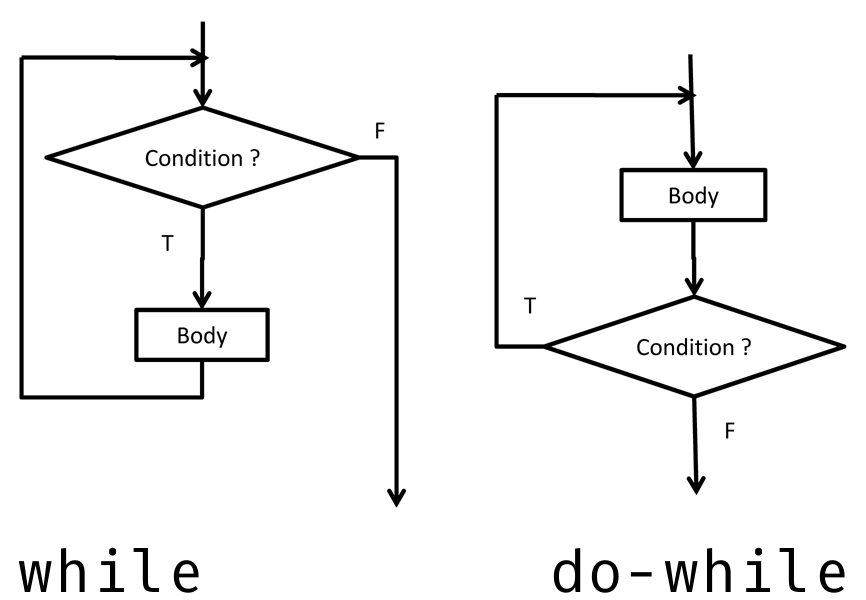
\includegraphics{img/while_vs_dowhile.jpg}
    \end{figure}
\end{frame}

\begin{frame}[fragile]{Schleifen: for}
    \begin{block}{}
        \textbf{Für} \textit{Zählvariable} \textbf{von} \textit{untere Grenze} \textbf{bis} \textit{obere Grenze}\\
        \textit{Anweisungen ausführen}\dots
    \end{block}
    \pause

    \begin{block}{}
        \begin{lstlisting}[language=Java]
for (int i = from; i < to; ++i) {
    instruction;
}
        \end{lstlisting}
    \end{block}
\end{frame}

\begin{frame}[fragile]{Schleifen: for}
    \begin{exampleblock}{}
    \begin{lstlisting}[language=Java]
for (int i = 0; i < 4; ++i) {
    System.out.println("Hallo aus for-Schleife!");
}
    \end{lstlisting}
    \end{exampleblock}
\end{frame}
%%%%%%%%%%%%%%%%%%%%%%%%%%%%%%%%%%%%%%%%%%%%%%%%%%%%%%%%%%%%%%%%%%%%%%%%%%%%%%%%%%%%%%%%%%%%%%%%%%%%%%%%%%%%%%%%%%%%%%%%
\begin{frame}[fragile]{Quiz: Was kommt raus?}
    \begin{exampleblock}{}
        \begin{lstlisting}[language=Java]
int counter = 5;

if (counter > 0) {
    System.out.println(counter);
}
        \end{lstlisting}
    \end{exampleblock}
\end{frame}

\begin{frame}[fragile]{Quiz: Was kommt raus?}
    \begin{block}{}
        \begin{lstlisting}
5
        \end{lstlisting}
    \end{block}
\end{frame}
%%%%%%%%%%%%%%%%%%%%%%%%%%%%%%%%%%%%%%%%%%%%%%%%%%%%%%%%%%%%%%%%%%%%%%%%%%%%%%%%%%%%%%%%%%%%%%%%%%%%%%%%%%%%%%%%%%%%%%%%
\begin{frame}[fragile]{Quiz: Was kommt raus?}
    \begin{exampleblock}{}
        \begin{lstlisting}[language=Java]
int counter = 5;

while (counter > 0) {
    System.out.println(counter);
}
        \end{lstlisting}
    \end{exampleblock}
\end{frame}

\begin{frame}[fragile]{Quiz: Was kommt raus?}
    \begin{block}{}
        \begin{lstlisting}
5
5
5
5
5
5
5
5
...
        \end{lstlisting}
    \end{block}
\end{frame}
%%%%%%%%%%%%%%%%%%%%%%%%%%%%%%%%%%%%%%%%%%%%%%%%%%%%%%%%%%%%%%%%%%%%%%%%%%%%%%%%%%%%%%%%%%%%%%%%%%%%%%%%%%%%%%%%%%%%%%%%
\begin{frame}[fragile]{Quiz: Was kommt raus?}
    \begin{exampleblock}{}
        \begin{lstlisting}[language=Java]
int counter = 5;

while (counter > 0) {
    System.out.println(counter);
    counter--;
}
        \end{lstlisting}
    \end{exampleblock}
\end{frame}

\begin{frame}[fragile]{Quiz: Was kommt raus?}
    \begin{block}{}
        \begin{lstlisting}
5
4
3
2
1
        \end{lstlisting}
    \end{block}
\end{frame}
%%%%%%%%%%%%%%%%%%%%%%%%%%%%%%%%%%%%%%%%%%%%%%%%%%%%%%%%%%%%%%%%%%%%%%%%%%%%%%%%%%%%%%%%%%%%%%%%%%%%%%%%%%%%%%%%%%%%%%%%
\begin{frame}[fragile]{Quiz: Was kommt raus?}
    \begin{exampleblock}{}
        \begin{lstlisting}[language=Java]
int counter = 5;

while (--counter > 0) {
    System.out.println(counter);
}
        \end{lstlisting}
    \end{exampleblock}
\end{frame}

\begin{frame}[fragile]{Quiz: Was kommt raus?}
    \begin{block}{}
        \begin{lstlisting}
4
3
2
1
        \end{lstlisting}
    \end{block}
\end{frame}
%%%%%%%%%%%%%%%%%%%%%%%%%%%%%%%%%%%%%%%%%%%%%%%%%%%%%%%%%%%%%%%%%%%%%%%%%%%%%%%%%%%%%%%%%%%%%%%%%%%%%%%%%%%%%%%%%%%%%%%%
\begin{frame}[fragile]{Quiz: Was kommt raus?}
    \begin{exampleblock}{}
        \begin{lstlisting}[language=Java]
int counter = 5;

while (counter-- > 0) {
    System.out.println(counter);
}
        \end{lstlisting}
    \end{exampleblock}
\end{frame}

\begin{frame}[fragile]{Quiz: Was kommt raus?}
    \begin{block}{}
        \begin{lstlisting}
4
3
2
1
0
        \end{lstlisting}
    \end{block}
\end{frame}
%%%%%%%%%%%%%%%%%%%%%%%%%%%%%%%%%%%%%%%%%%%%%%%%%%%%%%%%%%%%%%%%%%%%%%%%%%%%%%%%%%%%%%%%%%%%%%%%%%%%%%%%%%%%%%%%%%%%%%%%
\begin{frame}[fragile]{Quiz: Was kommt raus?}
    \begin{exampleblock}{}
        \begin{lstlisting}[language=Java]
int counter = 5;

while (counter > 7) {
    System.out.println(counter);
    counter--;
}
        \end{lstlisting}
    \end{exampleblock}
\end{frame}

\begin{frame}[fragile]{Quiz: Was kommt raus?}
    \begin{block}{}
        \begin{lstlisting}

        \end{lstlisting}
    \end{block}
\end{frame}
%%%%%%%%%%%%%%%%%%%%%%%%%%%%%%%%%%%%%%%%%%%%%%%%%%%%%%%%%%%%%%%%%%%%%%%%%%%%%%%%%%%%%%%%%%%%%%%%%%%%%%%%%%%%%%%%%%%%%%%%
\begin{frame}[fragile]{Quiz: Was kommt raus?}
    \begin{exampleblock}{}
        \begin{lstlisting}[language=Java]
int counter = 5;

do {
    System.out.println(counter);
    counter--;
} while (counter > 7);
        \end{lstlisting}
    \end{exampleblock}
\end{frame}

\begin{frame}[fragile]{Quiz: Was kommt raus?}
    \begin{block}{}
        \begin{lstlisting}
5
        \end{lstlisting}
    \end{block}
\end{frame}
%%%%%%%%%%%%%%%%%%%%%%%%%%%%%%%%%%%%%%%%%%%%%%%%%%%%%%%%%%%%%%%%%%%%%%%%%%%%%%%%%%%%%%%%%%%%%%%%%%%%%%%%%%%%%%%%%%%%%%%%
\begin{frame}[fragile]{Quiz: Was kommt raus?}
    \begin{exampleblock}{}
        \begin{lstlisting}[language=Java]
for (int i = 0; i < 4; ++i) {
    System.out.println("Hallo aus for-Schleife!");
}
        \end{lstlisting}
    \end{exampleblock}
\end{frame}

\begin{frame}[fragile]{Quiz: Was kommt raus?}
    \begin{block}{}
        \begin{lstlisting}
Hallo aus for-Schleife!
Hallo aus for-Schleife!
Hallo aus for-Schleife!
Hallo aus for-Schleife!
        \end{lstlisting}
    \end{block}
\end{frame}
%%%%%%%%%%%%%%%%%%%%%%%%%%%%%%%%%%%%%%%%%%%%%%%%%%%%%%%%%%%%%%%%%%%%%%%%%%%%%%%%%%%%%%%%%%%%%%%%%%%%%%%%%%%%%%%%%%%%%%%%
\begin{frame}[fragile]{Quiz: Was kommt raus?}
    \begin{exampleblock}{}
        \begin{lstlisting}[language=Java]
for (int i = 0; i < 4; ++i) {
    System.out.println("Hallo " + i);
}
        \end{lstlisting}
    \end{exampleblock}
\end{frame}

\begin{frame}[fragile]{Quiz: Was kommt raus?}
    \begin{block}{}
        \begin{lstlisting}
Hallo 0
Hallo 1
Hallo 2
Hallo 3
        \end{lstlisting}
    \end{block}
\end{frame}
%%%%%%%%%%%%%%%%%%%%%%%%%%%%%%%%%%%%%%%%%%%%%%%%%%%%%%%%%%%%%%%%%%%%%%%%%%%%%%%%%%%%%%%%%%%%%%%%%%%%%%%%%%%%%%%%%%%%%%%%
\begin{frame}[fragile]{Quiz: Was kommt raus?}
    \begin{exampleblock}{}
        \begin{lstlisting}[language=Java]
for (int i = 5; i > 0; --i) {
    System.out.println("Hallo " + i);
}
        \end{lstlisting}
    \end{exampleblock}
\end{frame}

\begin{frame}[fragile]{Quiz: Was kommt raus?}
    \begin{block}{}
        \begin{lstlisting}
Hallo 5
Hallo 4
Hallo 3
Hallo 2
Hallo 1
        \end{lstlisting}
    \end{block}
\end{frame}
%%%%%%%%%%%%%%%%%%%%%%%%%%%%%%%%%%%%%%%%%%%%%%%%%%%%%%%%%%%%%%%%%%%%%%%%%%%%%%%%%%%%%%%%%%%%%%%%%%%%%%%%%%%%%%%%%%%%%%%%

\begin{frame}{while vs. for}
    \begin{itemize}
        \item Jede \texttt{for}-Schleife kann auch als \texttt{while}-Schleife umgeschrieben werden und andersrum
        \pause
        \vspace{.3in}
        \item Typischerweise
        \begin{itemize}
            \item \texttt{for}-Schleife: hoch- bzw. runterzählen
            \item \texttt{while}-Schleife: allgemeine Bedingung
        \end{itemize}
    \end{itemize}
\end{frame}

\subsection{Unbedingte Sprünge}

\begin{frame}[fragile]{Unbedingte Sprünge:\\ break und continue}
    \begin{block}{}
        \begin{itemize}
            \item \texttt{break}: Verlasse Schleife
            \item \texttt{continue}: Überspringe aktuellen Schleifendurchlauf
        \end{itemize}
    \end{block}
\end{frame}

%%%%%%%%%%%%%%%%%%%%%%%%%%%%%%%%%%%%%%%%%%%%%%%%%%%%%%%%%%%%%%%%%%%%%%%%%%%%%%%%%%%%%%%%%%%%%%%%%%%%%%%%%%%%%%%%%%%%%%%%
\begin{frame}[fragile]{Quiz: Was kommt raus?}
    \begin{exampleblock}{}
        \begin{lstlisting}[language=Java]
for (int i = 1; i < 100; ++i) {
    if (i % 3 == 0 && i % 7 == 0) {
        System.out.println(i);
        break;
    }
}
        \end{lstlisting}
    \end{exampleblock}
\end{frame}

\begin{frame}[fragile]{Quiz: Was kommt raus?}
    \begin{block}{}
        \begin{lstlisting}
21
        \end{lstlisting}
    \end{block}
\end{frame}
%%%%%%%%%%%%%%%%%%%%%%%%%%%%%%%%%%%%%%%%%%%%%%%%%%%%%%%%%%%%%%%%%%%%%%%%%%%%%%%%%%%%%%%%%%%%%%%%%%%%%%%%%%%%%%%%%%%%%%%%
\begin{frame}[fragile]{Quiz: Was kommt raus?}
    \begin{exampleblock}{}
        \begin{lstlisting}[language=Java]
for (int i = 1; i < 100; ++i) {
    if (i % 3 == 0 && i % 7 == 0) {
        System.out.println(i);
    }
}
        \end{lstlisting}
    \end{exampleblock}
\end{frame}

\begin{frame}[fragile]{Quiz: Was kommt raus?}
    \begin{block}{}
        \begin{lstlisting}
21
42
63
84
        \end{lstlisting}
    \end{block}
\end{frame}
%%%%%%%%%%%%%%%%%%%%%%%%%%%%%%%%%%%%%%%%%%%%%%%%%%%%%%%%%%%%%%%%%%%%%%%%%%%%%%%%%%%%%%%%%%%%%%%%%%%%%%%%%%%%%%%%%%%%%%%%
\begin{frame}[fragile]{Quiz: Was kommt raus?}
    \begin{exampleblock}{}
        \begin{lstlisting}[language=Java]
for (int i = 1; i < 100; ++i) {
    if (i % 2 != 0) {
        continue;
    }
    if (i % 3 == 0 && i % 7 == 0) {
        System.out.println(i);
        break;
    }
}
        \end{lstlisting}
    \end{exampleblock}
\end{frame}

\begin{frame}[fragile]{Quiz: Was kommt raus?}
    \begin{block}{}
        \begin{lstlisting}
42
        \end{lstlisting}
    \end{block}
\end{frame}

\appendix

\beginbackup

\begin{frame}{Fragen?}
    \begin{figure}
        
\includegraphics[scale=.3]{img/fragen.jpg}
    \end{figure}
\end{frame}

\begin{frame}{Bis nächste Woche!}
    \begin{figure}
        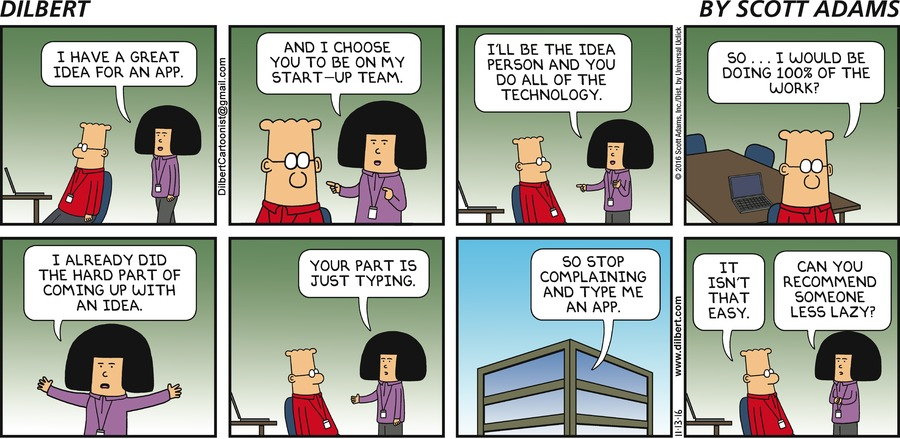
\includegraphics[scale=2.8]{img/dt161113.jpg}
        \caption{\footnotesize{dilbert.com}}
    \end{figure}
\end{frame}

\backupend

\end{document}
